%%%%%%%%%%%%%%%%%%%%%%%%%%%%%%%%%%%%%%%%%%%%%%%%%%%%%%%%%%%%%%%%%%%
%%% Documento LaTeX 																						%%%
%%%%%%%%%%%%%%%%%%%%%%%%%%%%%%%%%%%%%%%%%%%%%%%%%%%%%%%%%%%%%%%%%%%
% Título:		Capítulo 3
% Autor:  	Ignacio Moreno Doblas
% Fecha:  	2014-02-01, actualizado 2019-11-11
% Versión:	0.5.0
%%%%%%%%%%%%%%%%%%%%%%%%%%%%%%%%%%%%%%%%%%%%%%%%%%%%%%%%%%%%%%%%%%%
% !TEX root = A0.MiTFG.tex

\section{Quinta iteración: Consideraciones de diseño}
    \subsection{Resumen}
    
        Una vez teniendo el proyecto funcionando con todas las funciones básicas implementadas ha llegado el momento de frenar el desarrollo de nuevas funcionalidades y echar la vista atrás con el fin de mejorar el acabado general del proyecto.
        
        En esta iteración se llevarán a cabo tareas relacionadas con facilitar la lectura del código y mejorar el aspecto visual y usabilidad de la aplicación de usuario.
    
    \subsection{Requisitos}
    
        A diferencia de las anteriores, en esta iteración no se satisface ningún requisito en particular, pero igualmente se puede dividir el trabajo en las siguientes tareas.
        
        \begin{enumerate}
            \item Limpieza de código y asegurar coherencia en la nomenclatura.
            \item Añadir comentarios necesarios para facilitar la lectura del código y su mantenimiento.
            \item Mejorar la apariencia visual del panel y mejorar su usabilidad en la medida de lo posible.
        \end{enumerate}
        
        Además se aprovecha esta iteración de carácter finalizador para mejorar un apartado previamente desarrollado, la estimación del porcentaje de uso de la CPU.
    \subsection{Desarrollo}
    
        Para la primera tarea, \textit{revisar la limpieza del código y su coherencia}, se recorren los diferentes ficheros del código examinando con detalle el estilo de escritura utilizado, garantizando un código estandarizado y que satisfaga las consideraciones de diseño establecidas al comienzo del desarrollo.
        
       \textit{Comentarios explicativos} se han añadido a las declaraciones y demás elementos del código con el objetivo de facilitar la comprensión del mismo, especialmente en las zonas destinadas a ser modificadas por el usuario final. Además se han añadido comentarios referidos a posibles mejoras y correcciones que se podrían implementar en un futuro, por si el sistema sigue desarrollándose una vez concluido este proyecto. Minimizando así el tiempo de estudio previo a comenzar a realizar modificaciones.
       
       Para \textit{mejorar el apartado visual del panel} se han redistribuido los elementos ya expuestos en este proyecto, agrupándolos por secciones. Para \textit{mejorar la usabilidad} se han incluido textos descriptivos detallando a que corresponde cada elemento del panel y una nueva funcionalidad que permite detener el envío de una señal para realizar el análisis de otra sin la necesidad de reiniciar el panel. La nueva disposición de los elementos puede observarse en las imágenes \ref{fig:EndConfig} y \ref{fig:EndResults}.
        
        Con respecto al cálculo de uso de CPU, se ha decidido tomar un nuevo enfoque dado que las herramientas de medición del propio sistema operativo han demostrado ser muy ineficientes. Tanto en términos de rendimiento, ya que bloquean las interrupciones del procesador mientras se ejecutan, como en utilidad, ya que dadas sus limitaciones resultan poco precisas.
        
        Por estos dos motivos se ha decidido optar por calcular el uso de CPU de forma matemática, y aunque se trate de una aproximación en lugar de una medida, ya ha sido expuesta la inexactitud y la variabilidad de la medida realizada por el sistema, además se consigue quitar esa carga del procesador. 
        
        Para la estimación, la formula empleada ha sido:
        
        \begin{align*}
            \%CPU = \frac{f_{signal}*t_{algoritm}}{n_{samples} * F_{processor}} * 100
        \end{align*}
        
         Donde: \( f_{\mathrm{signal}}\) es la frecuencia a la que se envían las muestras de la señal, típicamente la frecuencia de muestreo a la que se tomó; \( t_{\mathrm{algorithm}}\) representa el número de operaciones o ``Ticks'' que emplea el algoritmo en ejecutarse, medido previamente en la tercera iteración; \( n_{\mathrm{samples}}\) el numero de muestras que se reciben antes de ejecutar el algoritmo, viene impuesto por el código y por defecto es ocho; Finalmente  \( F_{\mathrm{processor}}\) representa la frecuencia de trabajo del procesador, que indica el número de operaciones por segundo que este puede realizar.
         
          \begin{figure}[H]
            \centering
                    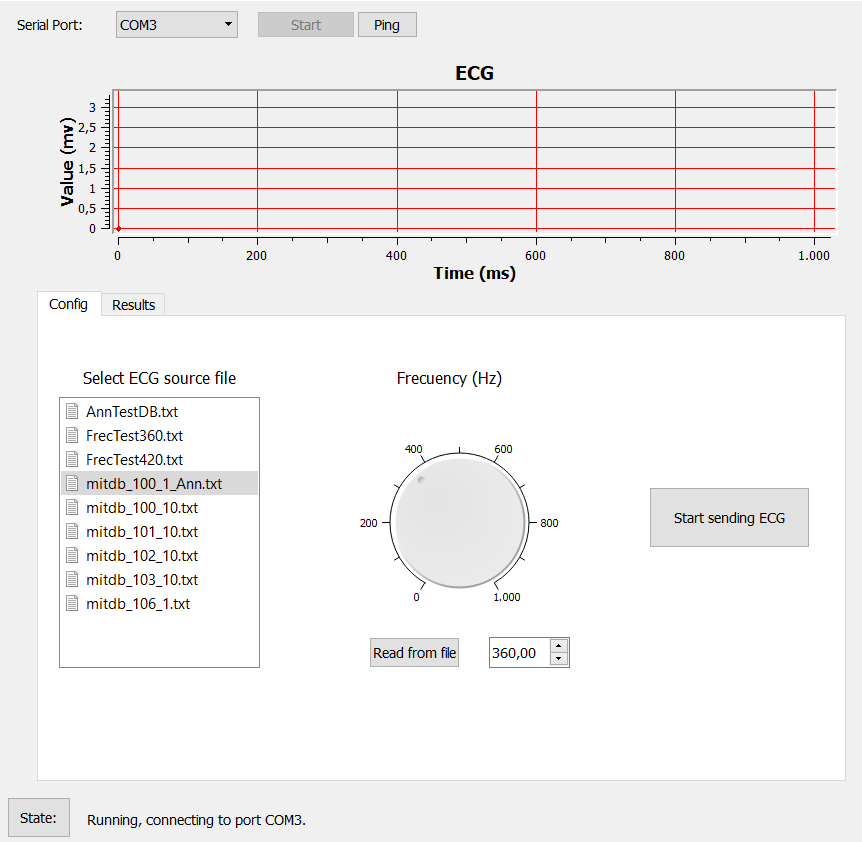
\includegraphics[width = \linewidth]{figuras/Config.PNG}
            \caption{Panel de usuario, configuración de la prueba.}
            \label{fig:EndConfig}
        \end{figure}
        
        \begin{figure}[H]
            \centering
                    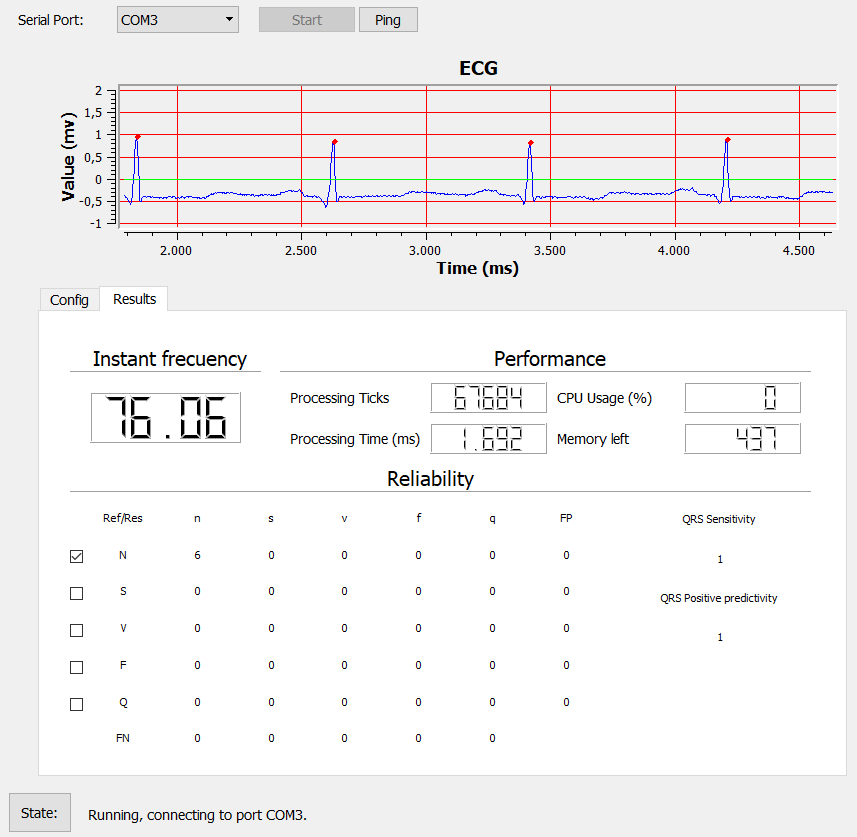
\includegraphics[width = \linewidth]{figuras/Results.PNG}
            \caption{Panel de usuario, resultados de la prueba.}
            \label{fig:EndResults}
        \end{figure}
        
    \clearpage
    \subsection{Pruebas}
    
    En esta iteración la única funcionalidad implementada susceptible de contener errores es la gestión del estado, necesaria para permitir al usuario detener y comenzar pruebas con diferentes muestras sin la necesidad de cerrar la sesión. Dado el carácter integral de esta funcionalidad resulta muy complicado realizar test unitarios, por lo que el método de prueba empleado ha sido simplemente un \textit{debug} intensivo probando exhaustivamente los casos posibles.
    
    \subsection{Conclusiones}
    
    Con esta iteración queda finalizado el desarrollo de este proyecto. El estado actual del sistema es estable, funcional y medianamente usable por lo que se pueden dar por finalizados todos los requisitos de alta prioridad establecidos al inicio del proyecto.
    
    A modo de resumen, a continuación se adjunta una tabla con los requisitos completos del proyecto, incluidos los que han surgido durante el desarrollo, y en ella se indica cuales se han satisfecho y cuales no.

 \begin{scriptsize}
    \begin{longtable}{|p{0.05\linewidth}|p{0.20\linewidth}|p{0.25\linewidth}|p{0.25\linewidth}|p{0.02\linewidth}|p{0.02\linewidth}|}
        \caption{Requisitos Finales. \label{tab:RequisitosFinales}}\\
        \hline
        ID & Requisito & Descripción & Prueba & Prio & Fin \\ \hline
        \endfirsthead
        %
        \endhead
        %
        \hline
        \endfoot
        %
        \endlastfoot
        %
        1 & Panel de control & El proyecto debe disponer de un panel de usuario intuitivo para llevar a cabo las pruebas &  & 1 & \\ \hline
        1.1 & Introducir señal de prueba & Al panel de control se le debe proveer una señal de ECG formateada específicamente para poder probar el algoritmo deseado & Introducir un ECG extraído de alguna base de datos y comprobar que los valores de las muestras enviados se corresponden & 1 & Si\\ \hline
        1.2     & Observar la señal procesada & Al panel de control se le debe proveer de una gráfica de salida que muestre la señal procesada. & Observar las gráfica de salida y comprobar que los datos dibujados se corresponden con los de la lectura & 2 & Si\\ \hline 
        1.3     & Resultados & El panel de control debe ser capaz de mostrar al usuario los siguientes elementos: &  &  & \\ \hline
        1.3.1   & Frecuencia cardiaca instantánea & El panel deberá mostrar la frecuencia cardíaca instantánea medida por el algoritmo a testear. & Comprobar que el dato enviado por la aplicación de pruebas y el recibido por el panel son el mismo. La precisión de este no es un requisito pues dependerá del algoritmo con el que se esté trabajando. & 1 & Si\\ \hline
        1.3.2   & Picos detectados & El panel deberá mostrar información sobre los picos R detectados y sus posiciones, para facilitar la evaluación del algoritmo & Al igual que la prueba anterior, se debe garantizar la coherencia de los datos entre la aplicación y el panel de usuario. La validez de estos dependerá del algoritmo. & 1 & Si\\ \hline
        1.3.3   & Utilización del procesador & El panel deberá mostrar el uso de CPU que corresponde al proceso del algoritmo de la forma más aproximada posible & Introducir una función con una duración conocida y realizar la estimación. & 1 & Si\\ \hline
        1.3.4   & Utilización de memoria & El panel deberá mostrar el uso de memoria en cada momento de la forma más aproximada posible & Introducir una función que consuma una memoria conocida y realizar la medición & 1 & Si\\ \hline
        1.3.5   & Fiabilidad del algoritmo visual & El panel deberá mostrar la fiabilidad del algoritmo de forma visual superponiendo los picos detectados con la señal en la gráfica. & Asegurar que los datos recibidos y dibujados son los mismos. La validez de estos dependen del algoritmo. & 1 & Si\\ \hline
        1.3.6   & Fiabilidad del algoritmo contrastada & El panel deberá mostrar la fiabilidad del algoritmo en forma de tasa de falsos negativos y positivos. & Contrastar los resultados con las anotaciones de la base de datos. & 2 & Si\\ \hline
        1.4     & Resolución muestras & El panel deberá poder configurar la resolución empleada para las muestras en la aplicación, ofreciendo al usuario cierto control sobre la cantidad de muestras simultaneas con las que su algoritmo podrá trabajar. & Comprobar la resolución de los valores y la cantidad de muestras totales a procesar con un inspector en modo \textit{debug}.  & 2 & No\\ \hline
        1.5 & Selección de datos & El panel deberá proporcionar al usuario un mecanismo por el cual pueda seleccionar de forma fácil e intuitiva el conjunto de muestras a emplear sobre sus pruebas & Comprobar que las muestras son tomadas y que se puede modificar la entrada de forma intuitiva. & 1 & Si \\ \hline
        1.6 & Mecanismo de mensajes & El panel deberá proporcionar al usuario información de los errores que se produzcan, además de manejarlos adecuadamente. & Forzar todos los errores conocidos y observar que la información mostrada al usuario es coherente & 2 & No \\ \hline
        2       & Dispositivo de pruebas & El sistema debe disponer de un dispositivo encargado de simular el comportamiento de un supervisor de eventos cardíacos que emplee el algoritmo de detección de tasa cardíaca deseado. &  & 1 & \\ \hline
        2.1     & Protocolo de comunicación & La aplicación debe ser capaz de recibir los datos desde el panel de usuarios y devolver los resultados procesados. & El correcto funcionamiento del resto de requisitos es prueba suficiente para este. & 1 & Si\\ \hline
        2.2     & Entrada de datos en tiempo real & La aplicación debe enviar y recibir los datos en tiempo real para emular las condiciones de funcionamiento de un SEC. & Comprobar que la aplicación es capaz de recibir datos paulatinamente y devolverlos. & 1 & Si\\ \hline
        2.2.1   & Simular la entrada de datos por el ADC & La aplicación debe simular la adquisición de datos mediante un conversor analógico digital. Emulando el funcionamiento de un supervisor real. & Comprobar que el acceso a esos datos está controlado con un \textit{timer}, como si del ADC se tratase. & 2 & No\\ \hline
        2.3     & Interfaz para el algoritmo & La aplicación debe disponer de una interfaz, dentro de la cual se pueda encapsular el algoritmo de detección de tasa cardíaca que el usuario desee probar. & Implementar dos algoritmos diferentes sin necesidad de modificar nada fuera de la interfaz. & 1 & Si\\ \hline
        2.4     & Resolución muestras & La aplicación debe ser capaz de modificar la resolución empleada para las muestras en la aplicación, ofreciendo al usuario cierto control sobre la cantidad de muestras simultaneas con las que su algoritmo podrá trabajar. & Comprobar que el máximo de muestras almacenadas en el dispositivo varían en función de la calidad seleccionada en el panel de control. & 2 & No\\ \hline
        2.5 & Aislamiento del procesado de señal & La implementación del algoritmo del usuario debe quedar encapsulada para facilitar las mediciones.  & Comprobar que el mecanismo de encapsulado se está empleando correctamente.  & 2 & Si \\ \hline 
    \end{longtable}   
    \end{scriptsize}
    
    Si bien hay aspectos del sistema que pueden ser mejorados y elementos que pueden añadirse, están fuera del alcance de este proyecto, aunque se hablará sobre ellos en las conclusiones generales del proyecto en un apartado posterior, así como de las tareas no finalizadas.